% Created 2022-04-15 Fri 13:21
% Intended LaTeX compiler: pdflatex
\documentclass[11pt]{article}
\usepackage[utf8]{inputenc}
\usepackage[T1]{fontenc}
\usepackage{graphicx}
\usepackage{longtable}
\usepackage{wrapfig}
\usepackage{rotating}
\usepackage[normalem]{ulem}
\usepackage{amsmath}
\usepackage{amssymb}
\usepackage{capt-of}
\usepackage{hyperref}
\usepackage{gensymb}
\usepackage{circuitikz}
\usepackage{tikz}
\usepackage{minted}
\usepackage[margin=2cm]{geometry}
\usepackage{fancyhdr}
\pagestyle{fancy}
\fancyhf{}
\fancyhead[L]{{\textcolor{gray}\leftmark}}
\fancyhead[R]{{\textcolor{gray}\thepage}}
\renewcommand{\headrulewidth}{0pt}
\usepackage{url}
\usepackage{rotfloat}
\usepackage{tikz}
\usepackage{float}
\hypersetup{hidelinks}
\usepackage{gensymb}
\usepackage{amsmath}
\numberwithin{equation}{section}
\usepackage{chngcntr}
\counterwithin{figure}{section}
\counterwithin{table}{section}
\usepackage{amssymb}
\newcommand {\R}{\mathbb{R}}
\usepackage{gensymb}
\usepackage{booktabs}
\usepackage{minted}[linenos]
\usepackage{sourcecodepro}
\definecolor{deepblue}{rgb}{0.0, 0.18, 0.39}
\setlength{\parindent}{0}
\usepackage{parskip}
\usepackage{enumitem}
\setlist{noitemsep}
\usepackage[format=plain, labelfont={bf}, textfont=it]{caption}
\usepackage{booktabs}
\usepackage[framemethod=tikz]{mdframed}
\BeforeBeginEnvironment{minted}{\begin{mdframed}[style=sourcecode]}
\AfterEndEnvironment{minted}{\end{mdframed}}
\author{Ben Frazer\thanks{2704250F@student.gla.ac.uk}}
\date{\today}
\title{The Future of UK Energy Mix}
\hypersetup{
 pdfauthor={Ben Frazer},
 pdftitle={The Future of UK Energy Mix},
 pdfkeywords={},
 pdfsubject={},
 pdfcreator={Emacs 27.2 (Org mode 9.6)}, 
 pdflang={English}}
\begin{document}

\maketitle
\tableofcontents

\mdfdefinestyle{sourcecode}{%
%backgroundcolor=darkgray,
skipabove=12pt,
hidealllines=true,
apptotikzsetting={%
  \tikzset{mdfbackground/.append style={fill=deepblue,fill opacity=0.1}}},
leftline=true,%innerleftmargin=10,innerrightmargin=10,
innerleftmargin=25,
linewidth = 4pt,
roundcorner = 2pt,
linecolor= darkgray,
%#frametitlerule=true,frametitlerulecolor=green,
%#frametitlebackgroundcolor=darkgray,
%#frametitlerulewidth=2pt
}
\section{Introduction}
\label{sec:org6c83099}
The UK government has committed to the target of becoming net zero by 2050. This commitment is just one of the many similar such commitments to net zero made by governments all around the world. In this essay I will explore how a truly zero carbon grid could be realised with only well established zero carbon technologies, and from this perspective highlight the fundamental trade-off and constrains which must be reconciled as a part of this transition. From this analysis a prediction will be made on the likely future prominent zero carbon technologies and what implication this mix will have on the grid.
\section{Current UK Energy Mix \label{secCurrentUkEnergyMix}}
\label{sec:org0e70717}
In 2020 UK annual electricity consumption was \(\approx\) \texttt{312TW}. Of this, roughly \(\approx\) \texttt{59.6\%} was generated from inherently carbon neutral sources (Nuclear/Renewables). Annual UK demand is broken down by generation technology in Figure \ref{figPie2020CumGen}, while carbon neutral energy generation is shown by relative energy generation in Figure \ref{figPie2020CumGen_all}.

\begin{figure}[H]
\centering
\includegraphics[width=0.8\textwidth]{./.ob-jupyter/442ca792c1e2256ccaf7ae3c93c0ece27e7708b3.png}
\caption{\label{figPie2020CumGen_all}Breakdown of UK energy Demand (Wave/tidal Excluded due to low scale) in GWh for the year 2020-2021 based on UK government data \cite{RenewableElecricityCap}}
\end{figure}

\begin{figure}[H]
\centering
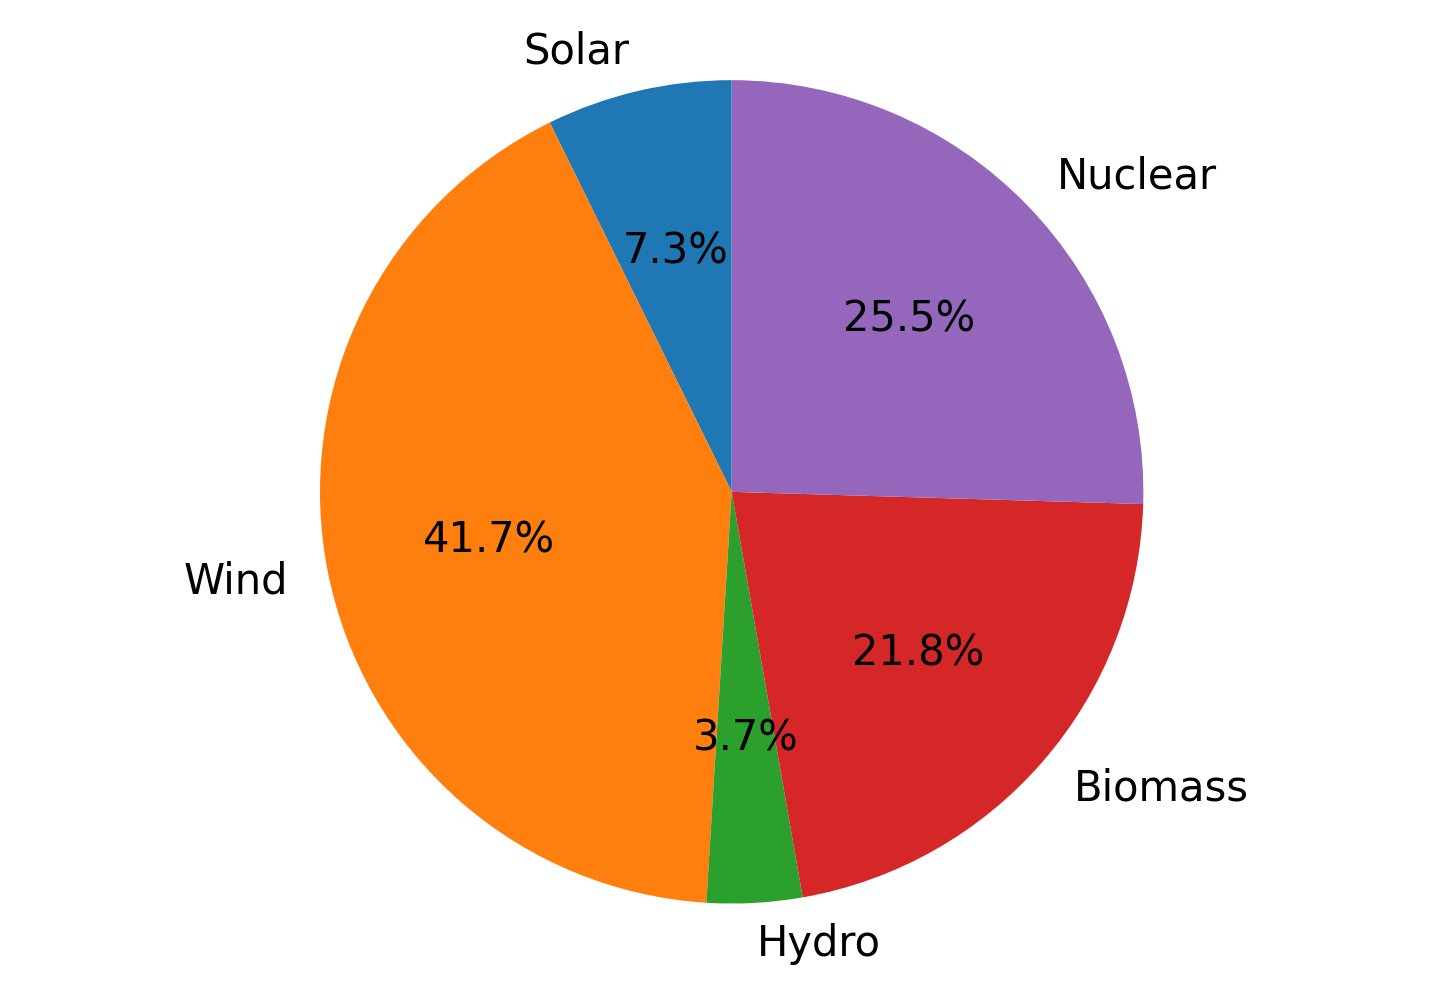
\includegraphics[width=0.8\textwidth]{./.ob-jupyter/9d5f54f66e0860cfcadd03202a7835f8eee375c2.png}
\caption{\label{figPie2020CumGen}Breakdown of UK zero carbon energy production (Wave/tidal Excluded due to low scale) in GWh for the year 2020-2021 based on UK government data \cite{RenewableElecricityCap}}
\end{figure}

\section{Capacity Factor (CF) \label{secCF}}
\label{sec:org9329733}
Capacity factor \footnote{Also known as load factor} is defined as the total energy generated over a period of time divided by the theoretical maximum as specified by it's nameplate rating.

\begin{align}
\label{eqCFDeff}
CF= \frac{E_{total}}{E_{max}}
\end{align}

CF is a useful high level metric and can be though of as the degree of utilisation of a given generator. Depending on the generation type, the capacity factor will vary due to factors such as:
\begin{itemize}
\item Intermittency of generation
\item Outages/Maintenance
\item Political incentivisation/dis-incentivisation
\item Curtailment due to overcapacity or network constrains
\end{itemize}

From Figure \ref{figCFBreakdown} we can see that capacity factor varies substantially between generation types. Wind and solar energy for example have a much lower CF than other generation. This can of-course be explained by the intermittent nature of the energy source, for example a wind turbine might be able to generate 8MW at high wind-speeds, however wind-speeds vary substantially throughout the day. Interestingly a noticeable difference exists between onshore and offshore wind, pointing to an advantage of offshore farms, that being greater consistence of generation.

Nuclear energy on the other hand has a relatively high capacity factor of \(\approx\)60\%\footnote{It should be noted that this capacity factor is substantially below the typical value which is often upwards of 80\% however given the ageing nuclear plants in the UK the past several years have seen substantial outages for maintenance, and plants coming offline.  In this sense this capacity should be seen as artifactualy low.}, this is largely because, as will be discussed further in Section \ref{secLCOEvsCF}, the key mechanism to lower cost of electricity is to increase CF.

\begin{figure}[H]
\centering
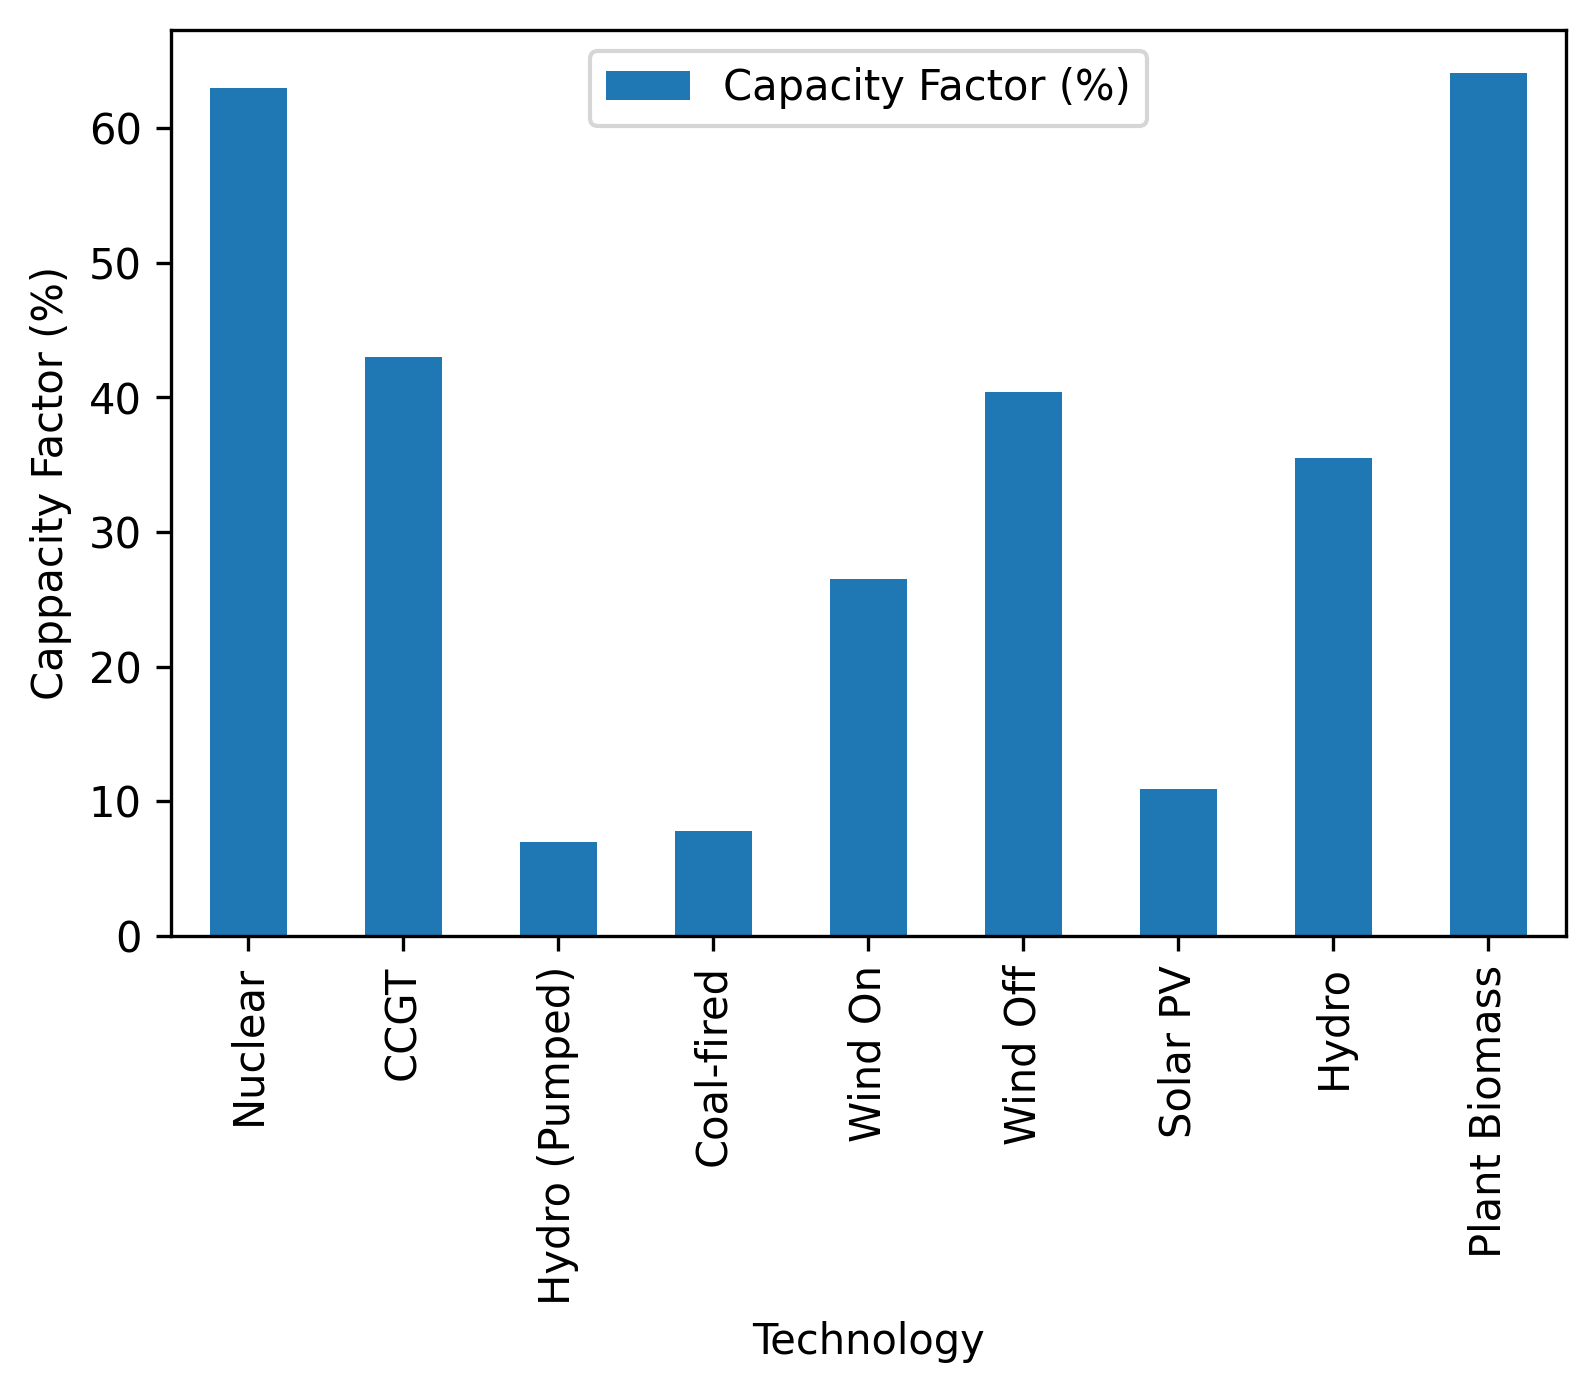
\includegraphics[width=0.8\textwidth]{./.ob-jupyter/8af7b171434f52c001534a44e0e1e32c5e7c5b94.png}
\caption{\label{figCFBreakdown}Breakdown of capacity Factor by Generation Type for 2019, Data Sourced from UK government \cite{NonRE_CF,RenewableElecricityCap}, Tabular data in Appendix Section \ref{secAppCFBreakdown}.}
\end{figure}
\section{Grid Stability Limitations of Converter based Generation \label{secInertiaLimmitsOfGeneration}}
\label{sec:org67264ae}
This section will attempt to give a brief overview of the limitations of converter based generation due to grid stability.

\subsection{Definition of Grid following}
\label{sec:org79e1658}
Developments in silicon power electronics, have enabled generators to interface with the grid without physically rotating machines. In a traditional synchronous machine, the back EMF is a product of the physically rotating magnetic field of the rotor, converters control their voltage by varying the duty cycle of power electronic switches at high frequency to create an average sinusoidal voltage. This has the advantage that the inverter voltage source, and as such the power flow, may be controlled with extremely high fidelity and bandwidth invariant to grid conditions.

This high bandwidth control gives the controls engineer the ability to completely reject almost any grid disturbance, and continue to operate only within the safe current of the device. For example, if a disturbance occurs such as a sharp fall in frequency, the converter will simply follow this frequency while exporting the exact same current. This is in contrast to a synchronous machine which will deliver inertial energy in proportion to the rate of change of frequency experienced according to the swing equation. The reasoning for designing this grid following characteristic is simple: Over rating components is expensive so instead the converter's operational envelope is limited.

Such grid follow converters to date make up the bulk off the installed capacity of renewable energy systems such as solar and wind farms.

\subsection{High Penetration of Grid Following Inverters}
\label{sec:org60424eb}
Penetration in the context of electrical networks is simply defined as the fraction of electricity generated by a given source of interest. As the network decarbonises, it is expected that the share of renewable energy sources has scaled up. Since much of this generation will be converter based, the UK grid is increasingly faced with situations in which the bulk of the connected generation are converter based. Since these devices can be thought of as non inertial, this has the effects of lowering the total system inertia.

\subsection{Synthetic Inertia With Renewables}
\label{sec:orgb89b220}
\subsubsection{Overview}
\label{sec:orgc9c6f02}
A technology under development that is targeted at addressing this is converter based inertia, referred to as 'synthetic Inertia' \footnote{Also referred to as Grid Forming and Virtual Synchronous Machine (VSM)}.

This algorithm aims to replicate the voltage source like behaviour of synchronous machines using a low bandwidth control of power, while the angle of the voltage sources is largely allowed to rotate according to the governing differential equations of a synchronous machine's rotor. Theoretically these converters will respond to frequency disturbances in much the same way as traditional synchronous machines within the operational envelope of the device.

\subsubsection{Benefits of synthetic Inertia}
\label{sec:org24671b9}
Since large scale penetration of grid following inverter based systems undermines network stability, it is increasingly likely that renewable generation will face increasing curtailment and/or national grid will be forced to compensate by increasing the deployment of mitigating techniques which will drive up the cost of electricity \footnote{Such mitigations have in the past included the installation of synchronous condensers or connecting non generating synchronous machines just for their stabilising effect}. In this sense, synthetic Inertia can be seen as both an enabler for higher renawable energy penetrations, and a means of lowering energy costs.

\section{Levelized Cost of Electricity (LCOE)}
\label{sec:orgecc1c46}
\subsubsection{What is LCOE}
\label{sec:orgdb15d9d}
Since we have established
Levelized cost of electricity (LCOE) is defined simply as the total cost of building, running and decommissioning an energy generation asset divided by it's lifetime generation cost.
\begin{align}
\label{eqLCOE}
LCOE = \frac{\text{Lifetime Cost (\$)}}{\text{Lifetime Production (KWh)}} = \frac{C_{Life}}{E_{Life}}
\end{align}

This is a vital metric for comparing the cost effectiveness and profitability of a given generation source. By accounting for profit margins and transmission/distribution use of system fees, this metric may also give a very rough insight into the likely end cost of energy to the consumer assuming a relatively competitive energy market.
\subsubsection{LCOE Breakdown by generation Type \label{LCOEBreakdown}}
\label{sec:orga005442}
\begin{figure}[H]
\centering
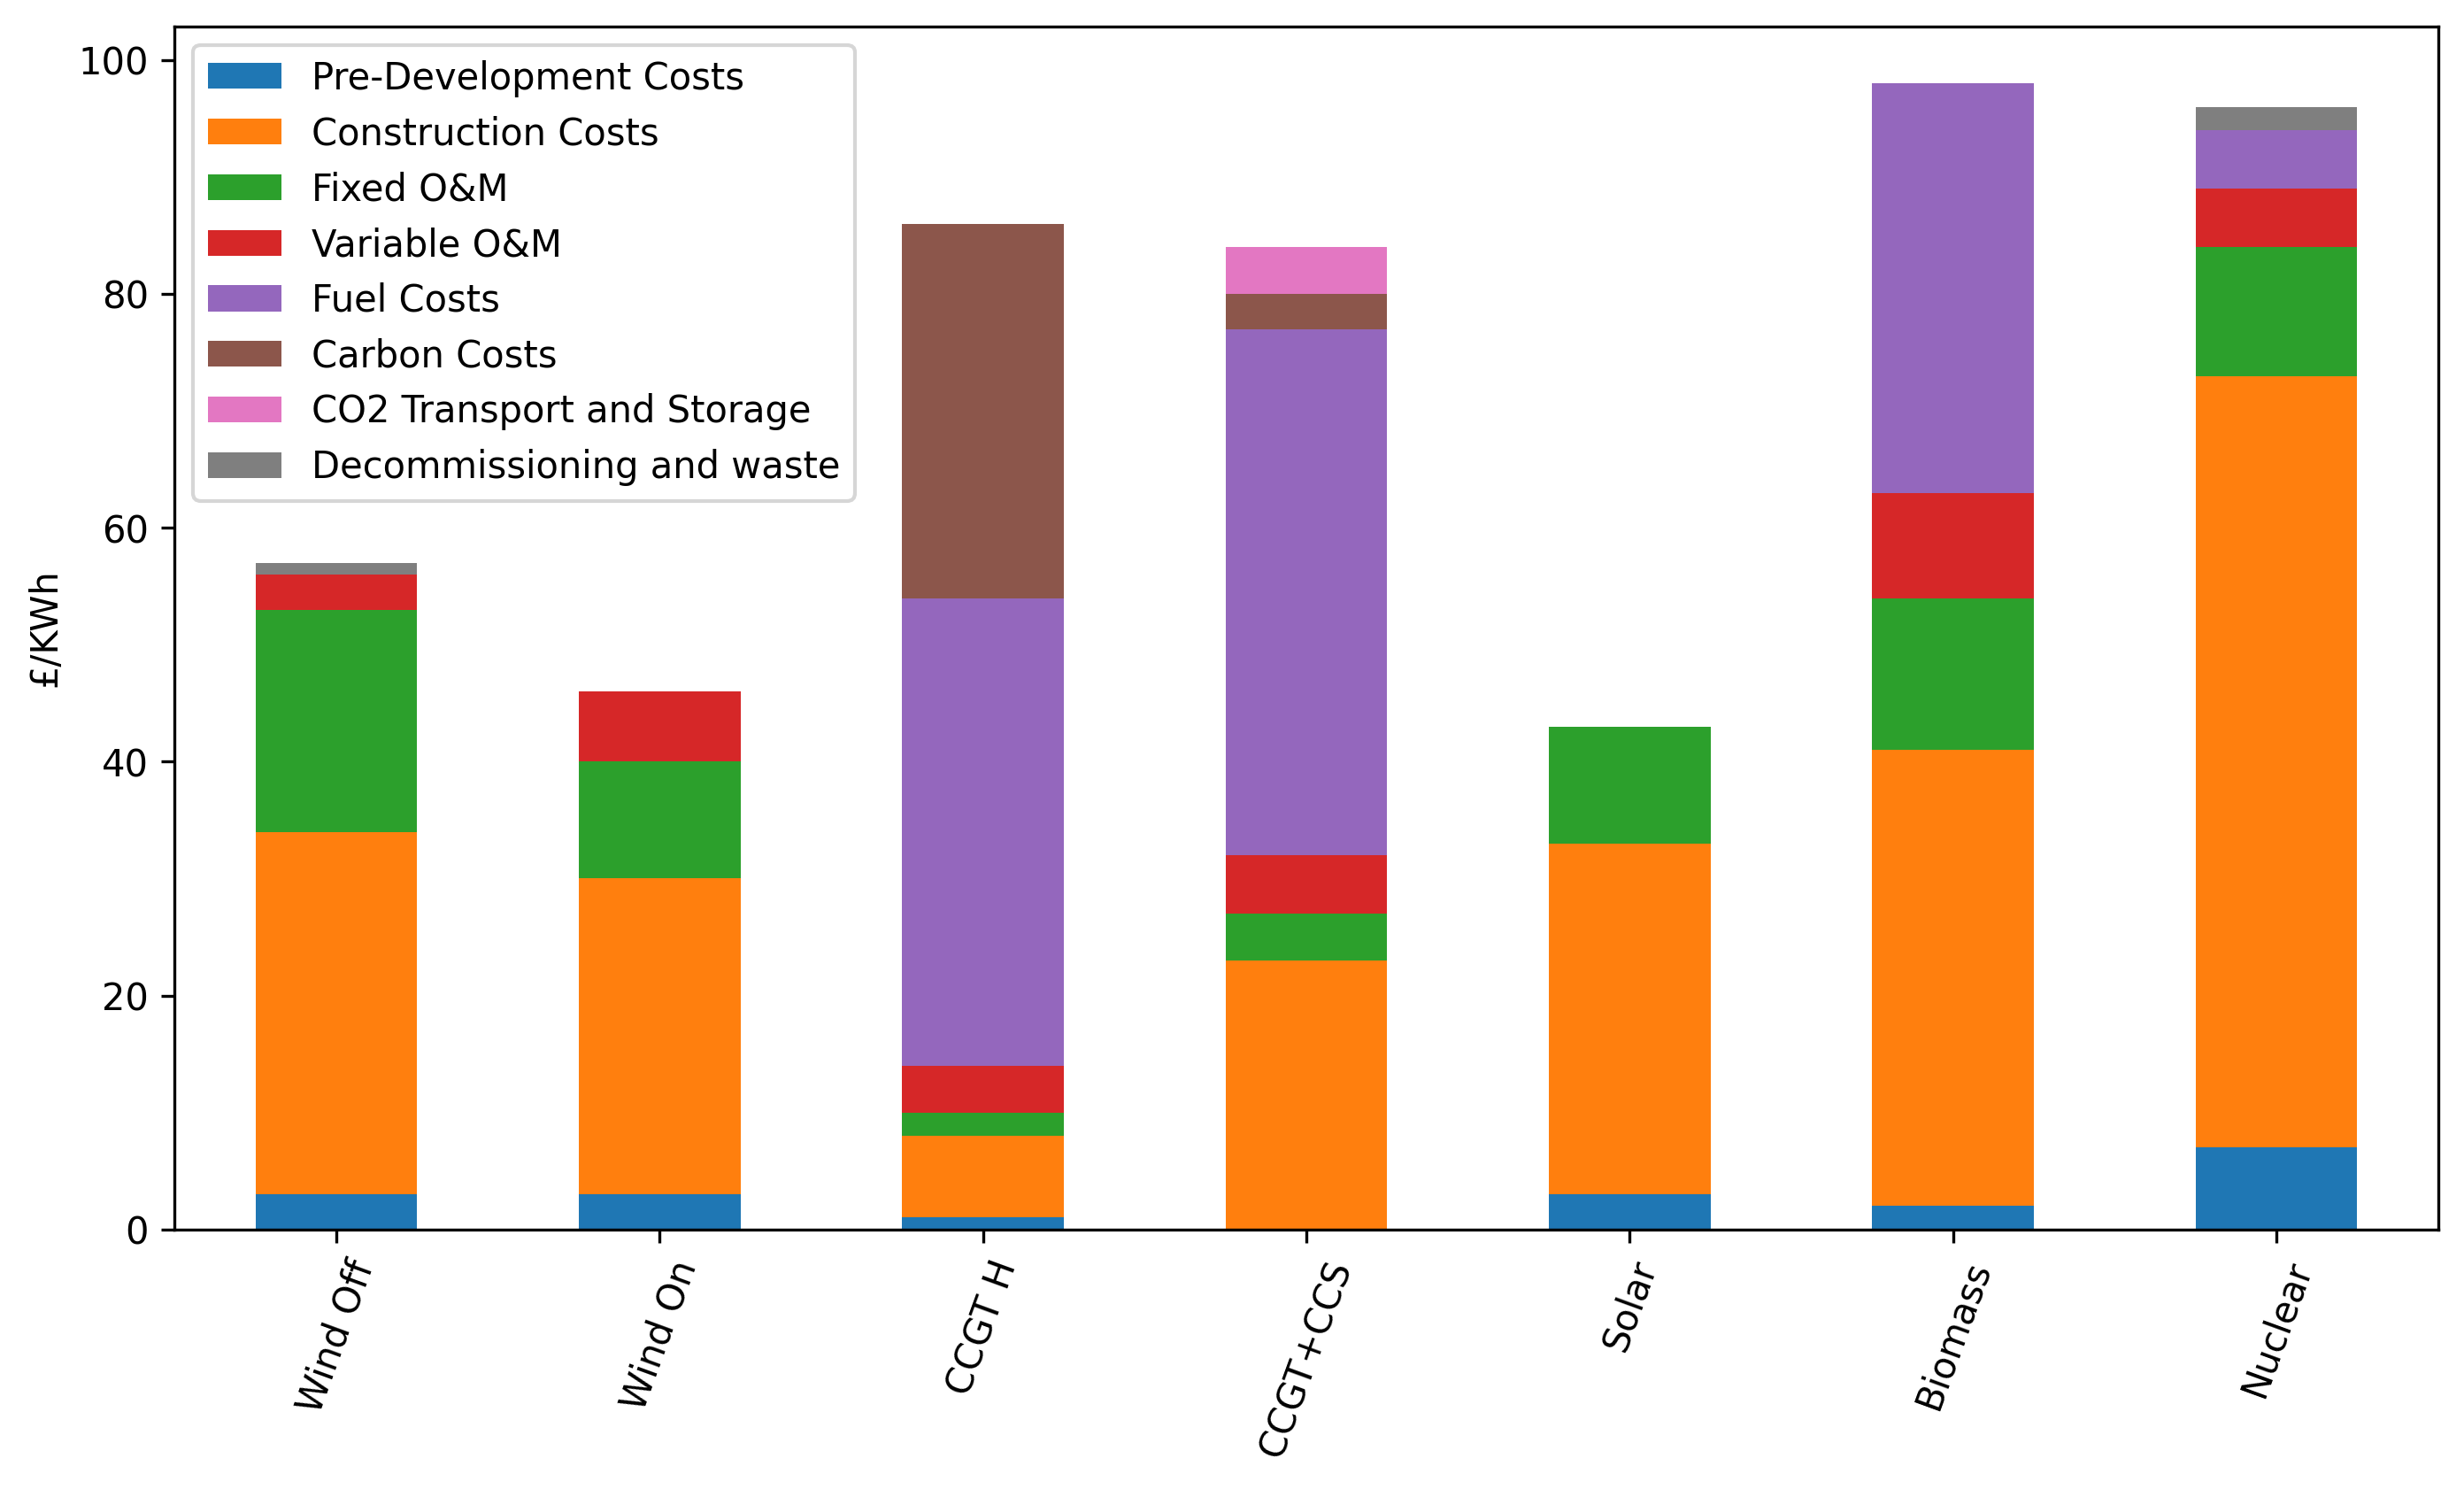
\includegraphics[width=0.8\textwidth]{./.ob-jupyter/8db2ae3ea8d23f67cdfb46f0d78029d25fe124bc.png}
\caption{\label{figLCOEbreakdown}Levelized cost Estimates for Projects commissioning in 2025, £/MWh (Data is sourced from UK Government Figures Published in 2020\cite{DeptEnerLCOE})}
\end{figure}

\subsubsection{LCOE vs Capacity factor \label{secLCOEvsCF}}
\label{sec:org647649d}
Choosing the optimal mix of energy generation is not simply a case of electing the lowest LCOE since the LCOE itself will be a function of the capacity factor and this capacity factor will be affected by the type of grid. This can be shown by assuming that the operational period (\(t_{hours}\)) and the levelized fuel cost is relatively fixed\footnote{It should be noted here that this is a very high-level analysis with many implicit assumptions, among them the assumption of fixed lifetime for a given generation type : This means that OEM costs which are roughly speaking a function of lifetime and capacity factor can be considered fixed costs.}, we can then rearrange Equation \ref{eqLCOE} into \ref{eqLCOE_5_final} (see Appendix \ref{secAppDerivationOfLCOEBreakdown} for full derivation).

\begin{align}
\label{eqLCOE_5_final}
LCOE &= \frac{C_{Fixed}}{S_{Base\; kW} \times t_{hours}\times CF}+ C_{Fuel(\pounds/kWh)} + C_{carbon(\pounds/kWh)}
\end{align}


Examining \ref{eqLCOE_5_final} see that generators trying to minimise LCOE roughly have only one degree of freedom \footnote{This ignores of course all of the other ancillary service which may be supplied on top of just energy.}, that being capacity factor. Indeed we see in generation like Nuclear energy where fixed costs are high and fuel +carbon costs are low, capacity factors are often very close to 1 and even then the LCOE is relatively high relative to other generation types (see \ref{LCOEBreakdown}). Wind and solar energy on the other hand have no fuel or carbon costs and relatively low LCOE, even with substantially lower capacity factors than other generation. This is because the cost per installed kW capacity (C\textsubscript{Fixed}) for wind and solar is so low that is compensates for this low CF.
\subsubsection{Seasonality Vs LCOE \label{secSeasonalityVsLSCO}}
\label{sec:org5f1504b}
The effect of seasonal variation on LCOE, can be derived by inspection of Equation \ref{eqLCOE_5_final}. To meet demand one must size capacity according to the peak demand effectively setting \(C_{Fixed}\) and \(S_{Base}\). One may assume these are linear with another so this has no impact on the LCOE. When the minimum in demand is substantially lower than the peak however, it necessarily lowers the system wide capacity factor and thus also increases the LCOE.

It should be noted here that where fuel is a dominant factor in the LCOE, there is less sensitivity to this lower capacity factor on the other hand, renewable generation is effectively inverse linearly dependant on CF.

\section{Future Space Heating Demand \label{secHeating}}
\label{sec:orgbbae687}
A critical challenges in the transition to net zero is decarbonising residential space heating. As of Tue, 15/03/22 the future of heating in the UK is still very unclear. Until recently the UK has relied on the abundant gas reserves of the north sea for the vast majority of it's heating needs. These reserves however are dwindling, and beyond being in carbon intensive, depending in imported natural gas is expected to incur increasing cost, not to mention poses a geopolitical vulnerability. It is thus no surprise that decarbonising heating has received substantial attention from the government.

The current policy of the UK government seems to be leaning in the direction of full electrification of heating using heat pumps in combination with altered building standards for improved insulation. This approach has been met with some scepticism on the grounds of high unit cost of heat-pumps and relatively limited uptake. It is the authors opinion however that these limitations may be mitigated though shared ownership of units or some form of district heating schemes.

Competing proposals have also been made to utilise the existing gas infrastructure instead with hydrogen generated through electrolyse rather than fossil fuel sourced gas \footnote{Biogas may also be used, however it seems unlikely that biogas will ever become a dominant source of heating due to fundamental limitations in available bio-matter}. This approach has the advantage of the relatively high energy density of hydrogen \footnote{This is relative to the current energy density of Lithium Ion battery} potentially allowing for relatively low cost energy storage. The potential advantages of hydrogen have also attracted significant attention in the transport sector, seeing research in cars, busses, trains and even boats. When competing with electrical storage such as batteries, or pumped hydro, it is still very unclear which, if any technology will decisively win-out in these sectors. If this were to occur,  it would likely substantial improve the economics of hydrogen for heating due to the potential to share infrastructure and in the benefits of research and commercial interest.

As such currently only two plausible scenarios exist for UK heating energy\footnote{It is noted that at least transiently, the end result will likely be some combination of both}:
\begin{enumerate}
\item Large scale Hydrogen gas network
\item Full Electrification using Heat-pumps
\end{enumerate}

When considered from the point of view of the electrical energy network, these two options are both fundamentally consumers of energy, however the quantity and distribution of the load vary substantially in each case.
\subsection{Current Natural gas demand \label{secCurrentNatGasDemand}}
\label{sec:orga0ce602}
Natural gas demand will be used as a proxy for the UK's current heating demand. In 2019 the UK's total natural gas demand was \(\approx\)863 TWh, of this, \(\approx\)377 TWh was in the domestic, commercial and public sector \cite{NaturalGas}. This report will assume that the majority of this energy is used for space heating, meaning that this figure is a good proxy for the UK's total space heating energy demand that must be decarbonized through electrical means.

From Figure \ref{figNatualGassDemandBreakdown} It is noted that this sector, though the largest, still only amounts to \(\approx\)43\% of total natural gas demand. With the exception of electrical generation, it is still largely unclear how many industrial uses of natural gas, for example the refinement of raw materials,will be decarbonised. A possibility is that net carbon syncs could trade their carbon capture capacity, or that these industries pivot towards zero carbon hydrogen. Both scenarios are likely to have substantial impacts on the network as a whole, however it is outwith the scope of this report to speculate future developments here so the influence of the remaining \(\approx\)25\% (Losses, Other and Industry) will not be considered.

\begin{figure}[H]
\centering
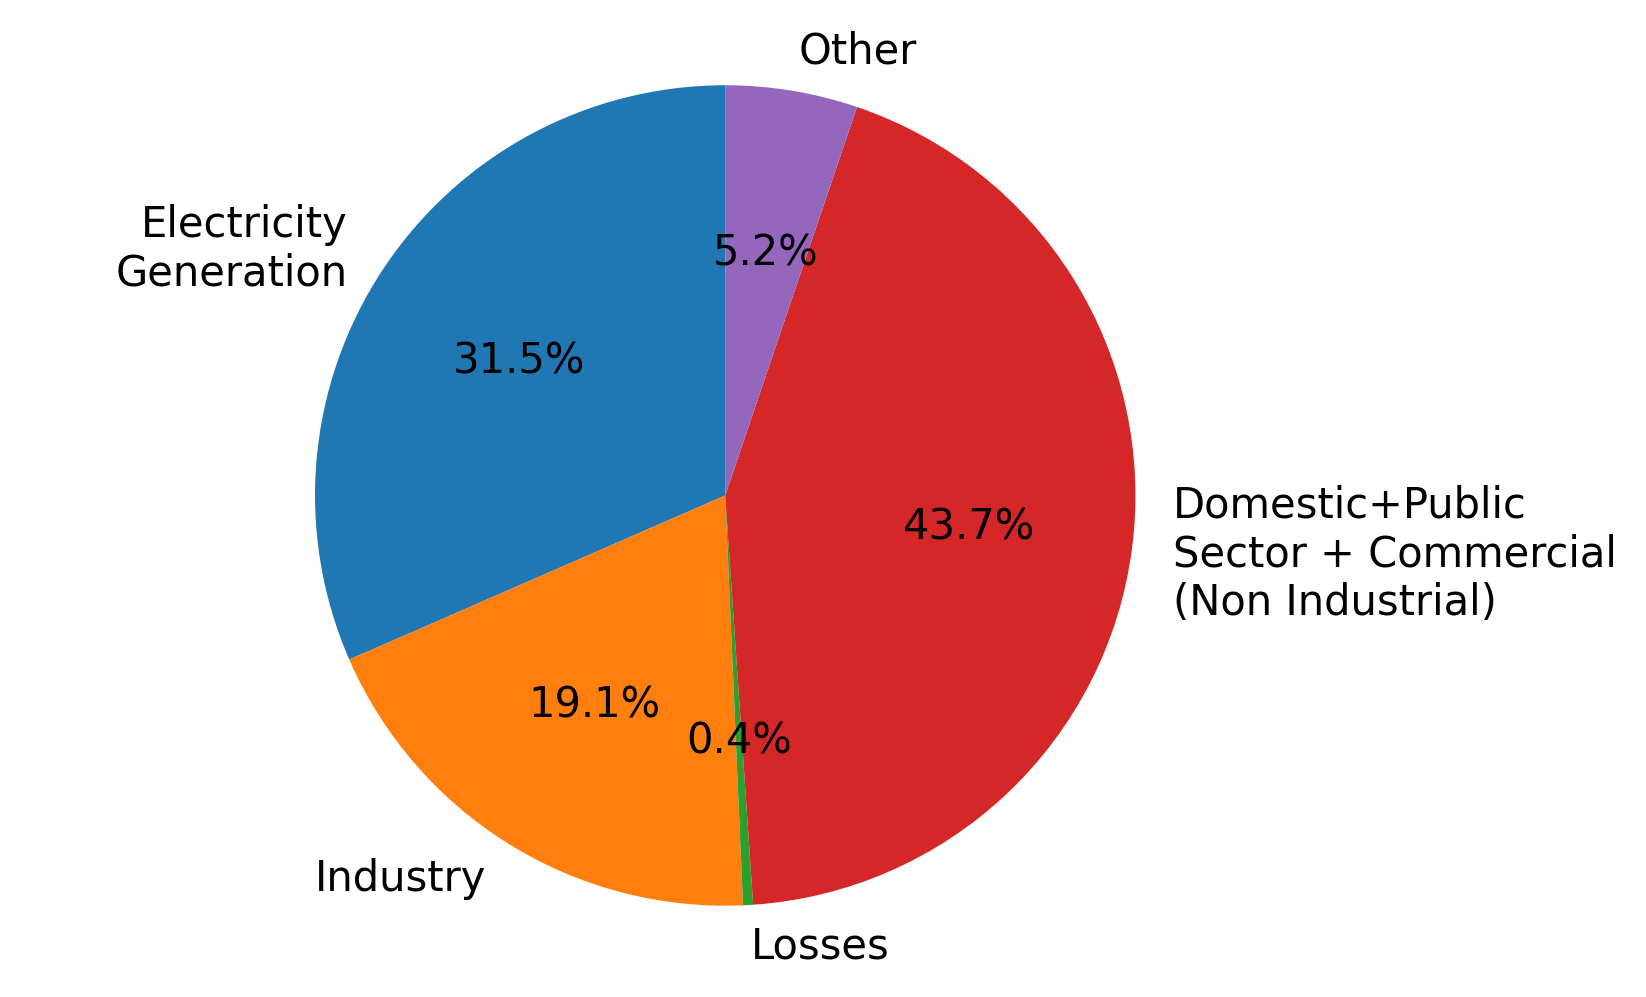
\includegraphics[width=0.8\textwidth]{./.ob-jupyter/059e5607973df26cf3fa1f5f9cae00619ccdfac7.png}
\caption{\label{figNatualGassDemandBreakdown}UK Natural Gas Demand for 2019, Figures supplied by the UK government \cite{NaturalGas}, Tabular Data in Appendix Section \ref{secAppNatGasDemand}.}
\end{figure}

\subsection{Electrical Characteristics of Hydrogen Scenario}
\label{sec:orgfb48712}
This section will briefly examine the implications of de-carbonisation of space heating using a purely hydrogen base approach.

\subsubsection{Hydrogen Energy Storage}
\label{sec:orga1f84a0}
The key advantage of hydrogen is of course the greater ease of storage\cite{HydrogenEnergyStorag2}. As such demand can be assumed to be dis-patchable to a certain degree, as long as the correct net energy is delivered. The option is also being discussed to attach
\subsubsection{Hydrogen Heating Electrical Energy Requirements}
\label{sec:org36002e4}
In the case of the large scale Hydrogen network, at least as much energy must be supplied electrically to the electrolyser producing the hydrogen fuel, as will be used by the consumer to heat. Since current alkaline fuel cell technology such as Cummin's HYDRLYZER can attain up to 70\% efficiency \cite{CuminsElectrolizer} and there will be other energy losses due to compression and leakage \footnote{Hydrogen tends to be substantially more leaky due to it's atomic size}, we may safely assume that the electrical energy required per unit thermal energy used will be at least \(\approx\) \texttt{1.5}.

Base on the current Natural gas space heating consumption inferred in Section \ref{secCurrentNatGasDemand}, we can estimate the expected future demand assuming a full adoption of this technology \footnote{This analysis is of course greatly simplified and makes a great many simplifying assumptions for instance: It is assumed that (despite plans to the contrary by the UK government) the space heating energy demand of the nation will remain roughly constant, though changes in building legislation aim to improve this on a per capita basis. This legislation will only be adopted in 2025, and then only apply to new builds, further more projections of the UK population grow forecast a rise of roughly 6.9\% by 2030. It seems likely therefore that for the foreseeable future, this demand will not deviate enough to invalidate this analysis.}.

\begin{align}
\label{eqFutureSpcHeatingDemand}
E_{Heating\;Electrical\;(kWh)} = 1.5\times E_{Heating\;Nat\;Gas (kWh)}
\end{align}

This yields and expected additional annual electrical load of \(\approx\) \texttt{565 TWh}, roughly \texttt{181\%} of the current annual electrical demand of \(\approx\) \texttt{312 TWh}. Restated, this would require an almost tripling in the UK's electrical energy generation capacity.

\subsection{Electrical Characteristics of Heat pump Scenario}
\label{sec:orgef00085}
\subsubsection{Coefficient of performance}
\label{sec:org1600351}
The coefficient of performance (COP) of a heat pump is defined as the ratio of useful heating to input energy.

\begin{align}
\label{eqCOPDef}
COP &= \frac{|Q_H|}{E_{in}} = \frac{Q_C+E_{in}}{E_{in}}\\
E_{in} &= \frac{Q_H}{COP}
\end{align}

Where \(Q_C\) is the heat moved from the cold reservoir \(Q_H\), is the total useful heating energy and \(E_{in}\) is the input energy.

Typical heat-pumps have COP in the range of 2-4 though the minimum to qualify for UK incentives is \texttt{2.9} this figure will be used as a base case in the subsequent analysis though it is expected that this figure will improve.

\subsubsection{Heat-pump Electrical Energy Requirements}
\label{sec:org0ffe57b}
Again using the figure for annual UK space heating demand derived in Section \ref{secCurrentNatGasDemand} (\texttt{565 TWh}) and Equation \ref{eqCOPDef}, we can estimate the additional electrical requirement as \(\approx\) \texttt{195 TWh}, roughly \texttt{62\%} of the current annual UK energy consumption. Note that this is not simply a case of adding an additional 62\% capacity, to the network due to the substantial seasonal variability in natural gas demand that will be discussed in Section \ref{secSpaceHeatingVariablity}.

\subsection{Seasonality of Demand \label{secSpaceHeatingVariablity}}
\label{sec:org1c4517d}
A key characteristic of heating demand however is it's inherent seasonality (shown in \ref{figHeatingSeasonality}) with peaks in demand often in excess of 5 times the minimum summer demand. This is a highly variable demand relative to the relatively stable variations in Electrical demand. Even with the factor of 2.9 reduction gained through the use of the heat pump, it is clear just by inspection of Figure \ref{figHeatingSeasonality}, that this seasonal spike in demand will require substantially more than just an increase in capacity of 62\%.

\begin{figure}[H]
\centering
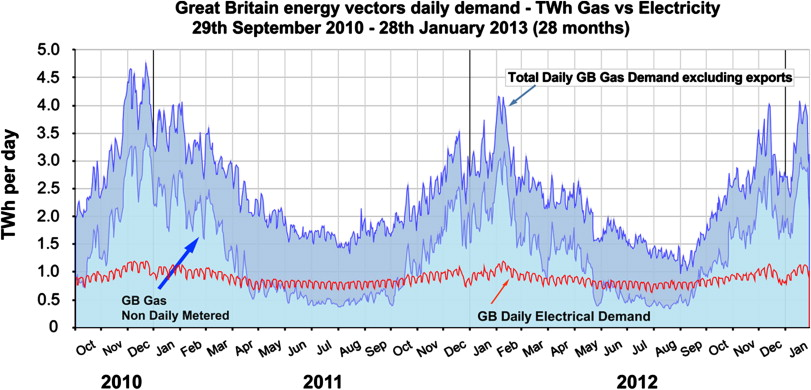
\includegraphics[width=0.8\textwidth]{Figures/SeasonalEnergyVariation.jpg}
\caption{\label{figHeatingSeasonality}Total daily GB Natural gas and Electricity usage, 29\textsubscript{th} Sept 2010 - 20\textsubscript{th} Jan 2013, (Source:\cite{ukNatGasAndElecConsumption})}
\end{figure}

\subsection{LCOE Constrains}
\label{sec:orgc91ccba}
A key constraint that policy makers will face, when attempting to address the de-carbonisation of electrical energy, is doing so without substantially increasing the cost of heat for the consumer. This naturally places a fundamental limit on the generation over capacity that may be installed since this will lead to higher LCOE due to lower CF. Further more, it is doubtful that energy storage based schemes

\subsubsection{Breakdown of an energy Bill}
\label{sec:orga73b214}
A vital constrain when considering future energy mix is that the cost of electricity to the end user remain low enough so that consumers will have manageable heating bills. This means that on a \$/kWh\footnote{\$/kWh is used for compatibility with the academic literature} heat energy must cost less than or in the region of the existing cost of gas. From this and the typical COP of a consumer grade heat pump, an upper limit on the acceptable cost per kWh may be established. This can then be roughly translated in an upper limit on the total LCOE of the generation sources on the network. From Figure \ref{figPieBillBreakdown}, we can see that the wholesale price of electricity, accounts for only \(\approx\)30\% of the final bill.

\begin{figure}[H]
\centering
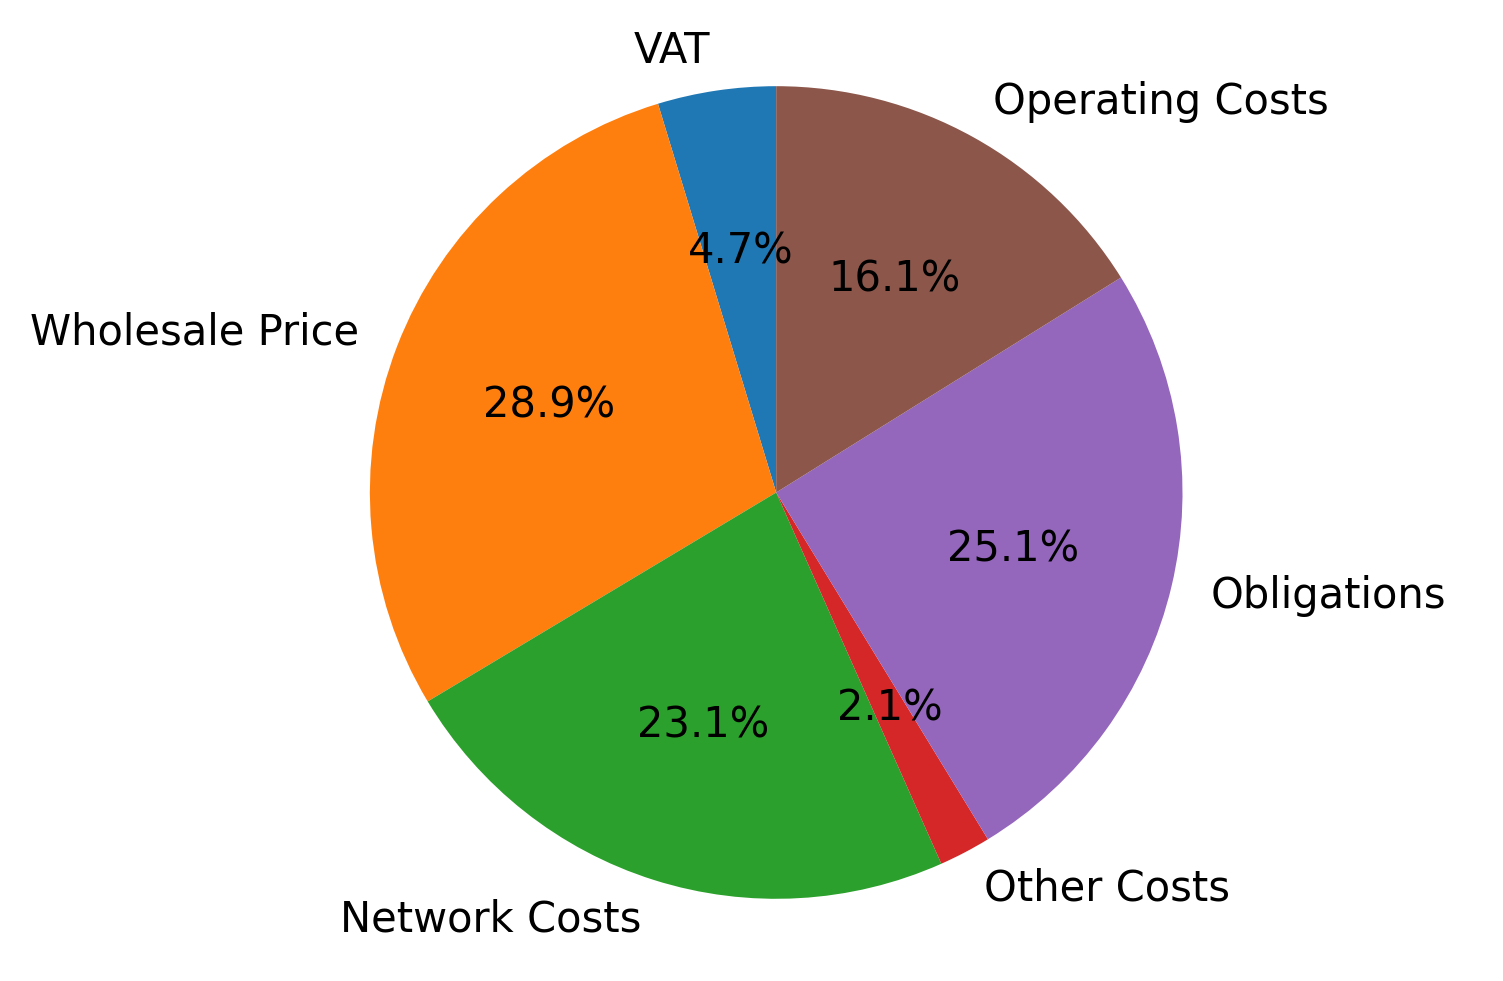
\includegraphics[width=0.8\textwidth]{./.ob-jupyter/78297f61231fd227439826e32eae830f0efb85e3.png}
\caption{\label{figPieBillBreakdown}Ofgem Estimated components of customer's energy bills from Ofgem \cite{ofgemBillBreakdown}}
\end{figure}

\subsection{Summary}
\label{sec:org576b664}
This degree of seasonal demand is something that has never been required of the electrical network before, and as discussed in Section \ref{secSeasonalityVsLSCO}, will necessarily lead to a rise in LCOE. It is the author's opinion, that the de-carbonisation of heating poses one of, if not the most substantial barrier to the UK's net zero plans.

\section{Predicted Future Zero carbon Energy Mix}
\label{sec:orgb6a7e0b}
Forecasting the future energy mix is the subject of extensive debate and is sensitive to a huge variety of unpredictable factors and unknowns such as government policy, geopolitical developments, to disruptive technologies. This analysis attempts to reason how a zero carbon grid might look with current technologies. A simplifying assumption made here is to exclude all fossil fuels from consideration although they may be modified to lower emissions substantially using so called carbon capture technology. The reasoning for this is simply that fossil fuels are fundamentally a finite and dwindling resource and as such humanity will need to learn to live without it sooner or later.

This section will investigate which combination of technologies would likely provide the bulk of energy in this future zero carbon grid. The technologies considered will be limited to the current widely adopted sources of renewable and zero carbon energy on the UK grid (shown in Figure \ref{figPie2020CumGen}) and use established performance figures rather than speculative future developments.

\subsection{Solar \label{secSolar}}
\label{sec:orgff970f7}
Off all dominant generation technologies, solar PV currently has the lowest LCOE, at roughly \texttt{45 £/kWh} according to \cite{DeptEnerLCOE}. Installation costs of solar PV having fallen by approximately 82\% between 2010 and 2020, and are expected to fall further still, meaning that solar PV will certainly remain a contester in the future energy mix.

\subsubsection{Limitations and Advantages}
\label{sec:org9601c2b}
A key constraint of solar PV is of course the inherent intermittency of supply due to weather and season. The UK, due to it's latitude, has substantial seasonal variability in it's day length and thus it's solar productivity. Further more, the UK's climate is such that (as discuss in Section \ref{secCurrentNatGasDemand}) the future energy network will expect the bulk of it's demand in the winter months when the generation from solar is at it's minimum.

Solar PV is inherently converter based generation and as such acts to reduce network stability as discussed in Section \ref{secInertiaLimmitsOfGeneration}. It is also likely, given the inherent lack of stored energy present in solar systems\footnote{unlike wind generation with stored energy in the blades.}, that solar converters would be a particularly good candidate for a \emph{synthetic inertia} algorithm. This means that solar PV will be likely to face substantial curtailment should capacity grow substantially.

The solar generation is also much more highly statistically across the country than say wind generation. For example a sunny day in Glasgow is more likely to predict a sunny day in London, than a windy day in London is to predict a windy day in Edinburgh. This is exacerbated further of course by the rigid seasonal and daily profile of solar PV. Since the quantity of incident solar Irradiance is so heavily influenced by cloud cover, this leads to huge and rapidly changing variability in generation. All of this conspires to a situation where the periods of peak generation is actually where the energy is least needed. While this instantaneous limitation of solar PV may be circumvented with energy storage, the network would still need to be sized to meet the greatest winter energy demand with little to no contribution from solar PV. If such were the case then this same generation should also be able to meet demand at the height of summer when demand is lower making solar PV obsolete.

\subsubsection{Summary}
\label{sec:org338aee9}
In summary, it is the author's view that solar PV makes sense in the UK only as a short term transitional technology, where solar energy may be used to transiently displace fossil fuels. It should be noted that this only works where rapidly dis-patchable generation such as natural gas exists on the network which can soak up the transient peaks and troughs.  Short of the cost of solar PV falling to the point that it becomes economical to operate solely on a winter capacity factor it seems unlikely that solar PV can scale to be the dominant generation source for a fully decarbonised grid \footnote{It is noted here that this dynamic may be drastically different in lower latitude countries where the dominant loads are air conditioning, and thus peak during the summer, and seasonal variability in generation is lower.}.

\subsection{Offshore Wind \label{secOffshoreWind}}
\label{sec:orgf6975b5}
Similar to solar PV, offshore wind is intermittent converter based generation. Estimates vary, but over the last decade the levelized cost of electricity from offshore wind has also decreased between 10-30\% and is projected to continue to do so.

\subsubsection{Limitations and advantage}
\label{sec:org901241b}
Due to the converter based nature of offshore wind farms, similar constraints apply to those discussed in Section \ref{secSolar}. However unlike solar the consistency of generation from offshore wind is much greater than that of solar, as can be seen by the fact that capacity factor for offshore wind is nearly four times higher than shown in Figure \ref{figCFBreakdown}. This makes intuitive sense, since wind is not nearly as affected by season or time of day as sunlight. Further more it can be shown that the level of correlation between wind-speed at individual sites diminishes rapidly, meaning that it is less likely that large numbers of wind farms are concurrently experiencing low wind at the same time.

Since the inverters used in the wind industry are typically on the order of MW and the spinning blades act as a source of energy storage, wind energy will likely be much more suitable for \emph{synthetic inertia} (see Section \ref{secInertiaLimmitsOfGeneration}).

\subsubsection{Summary}
\label{sec:org24afc3b}
All of this means that though the existing LCOE of offshore wind is substantially higher than that of solar PV, when the and costs problems associated with scaling competing generation technologies are accounted for, offshore wind compares very favourably.

\subsection{Nuclear}
\label{sec:org8430523}
Of the carbon neutral technologies present in the current UK energy mix, Nuclear energy has one of the highest LCOE at roughly \texttt{95 £/kWh} (see Section \ref{LCOEBreakdown}). Nuclear energy benefits from very low fuel costs (see Figure \ref{figLCOEbreakdown}) with the dominant costs coming from construction. From Figure \ref{figCFBreakdown} (Section \ref{secCF}) we see that Nuclear energy's capacity factor (\(\approx\) \texttt{60-70\%}) is already amongst the highest of all generation types.

\subsubsection{Limitations}
\label{sec:org7013eeb}
As with many of the prior technologies discussed, the limitations to scaling up nuclear energy primarily relate to the LCOE and as such the end cost to the consumer.  Given the already high LCOE, the low fuel costs and high construction costs, it is clear that minimising maintaining high capacity factors is vital to avoid large consumer electricity bills.

This poses problems when considering an energy network primarily supplied by nuclear energy, since the expected seasonal variability in demand incurred by the electrification of heating will doubtless eat substantially into the capacity factor causing a substantial increase in consumer energy bills.

Further more nuclear power ramps up and down generation with a relatively long time constant. This means that frequency regulation has and will need to continue to be the domain of either faster acting generation, or energy storage of some description.

\subsubsection{Advantages}
\label{sec:org1b8693f}
Nuclear energy's key advantage is it's consistent and predictable generation profile. Further more, nuclear energy along with hydro are amongst the only generation technologies that utilise synchronous machines and as such provide electrical inertia to the grid.

\subsubsection{Summary}
\label{sec:org9481912}
With it's consistent availability of supply and the inertia provided to the grid, it seems that Nuclear energy capacity will likely continue to grow. Due to the expected increased seasonality of demand, and the effect this will have on LCOE, it seems unlikely, short of a massive drop in the costs associated with nuclear energy, that it will become the single dominant generation technology.

\subsection{Biomass \label{secBioGas}}
\label{sec:org2a34224}
This section will be concerned with exploring the scalability and potential role that biomass may play in the future energy mix. For clarity, ``biomass'' in this essay will refer to a subset of generation types which produce energy from once living organisms \footnote{Note recently living i.e. not fossils} either by direct combustion or by generating gas through anerobic digestion.

A breakdown of the various technologies that constitute biomass energy is shown in Figure \ref{figPie2020BiomassBreakdown}. The reader should note that the totality of this chart represents only roughly \texttt{12.6\%} of the total UK electrical energy production that energy in the year 2020 \cite{BiomassPolicyStatement}. Many of these technologies vary substantially in their scalability however only the dominant form (plant biomass) will be considered here in this report.

\begin{figure}[H]
\centering
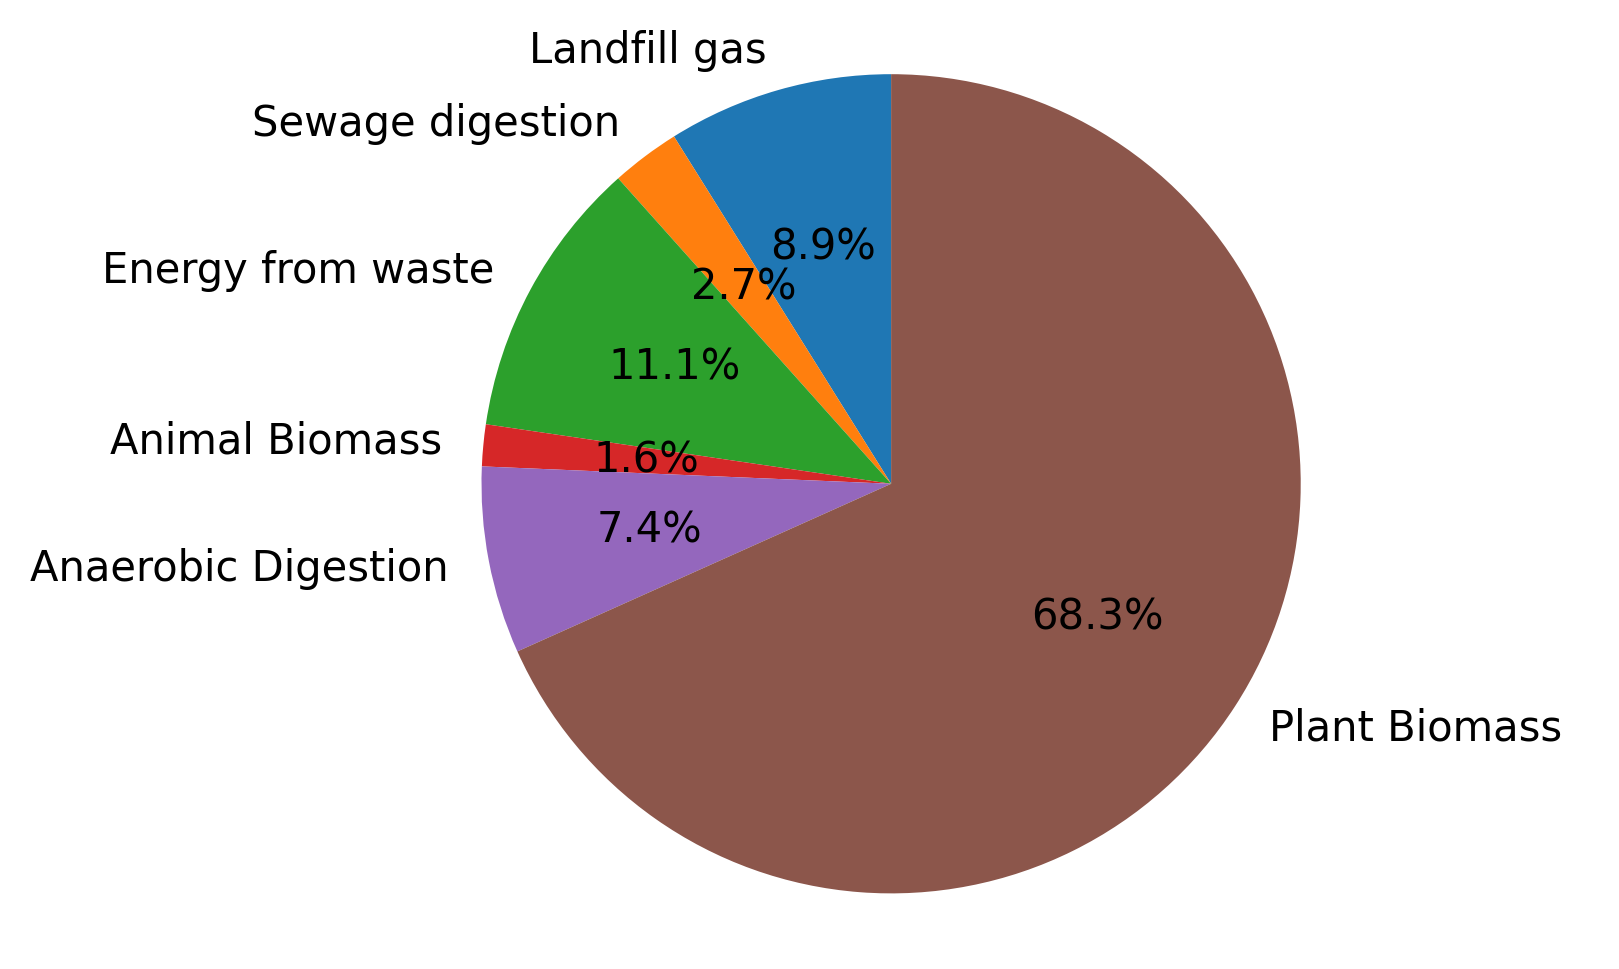
\includegraphics[width=0.8\textwidth]{./.ob-jupyter/7fa8fd63b7c93210e8cc642d47606e1527c98a39.png}
\caption{\label{figPie2020BiomassBreakdown}Breakdown of ``biomass'' energy by type based on UK government data \cite{RenewableElecricityCap} (For tabular data see Section \ref{secAppBiomassWasteEner})}
\end{figure}

\subsubsection{Plant Biomass Combustion}
\label{sec:orga208cca}
Plant biomass combustion is by far the dominant form of Biomass generation in the UK accounting for \(\approx\)68.3\% of total Biomass energy in the year 2020. The vast majority of this is in the form of wood bi-products and pellets imported from the united states and Canada \cite{BiomassPolicyStatement}.

Drax power plant is the largest biomass power plant in the UK, accounting for the vast majority of the UK's bio-energy production. The power station has six 660MW units, four of which were converted to purely biomass in 2016 yielding a total biomass capacity of 2.6GW. With the UK government's policy to phase out coal power by 2024 various plans were made to convert the remaining two units to gas and install carbon capture technology, however due to limited interest from the government, both plans have failed \cite{EndtoCoal2024}.

In theory, using such bio-fuels is net carbon neutral since the trees are harvested from managed woodlands which will regrow and recapture the emitted carbon, however there have been serious concerns raised about the transparency and traceability of the suppliers of these wooden pellets.

\subsubsection{Scalability}
\label{sec:org6fa0ccc}
Currently the UK based biomass schemes are heavily reliant on foreign imported feedstock in the form of wood pellets. Indeed, Drax is the larges single buyer of such wooden pellets in the world. Not only does the shipping of these pellets incur carbon emissions, it also hints at another inherent limit of this technology, that being land surface area. With the large majority of the UK being farmland, only around 13\% remains as forest, amounting to around 3.23 million hectares. The UK is already heavily dependant on foreign timber for the building sector, and wooden pellets imports have currently eclipsed these as the dominant import at 9.1million Tons \cite{ForestResearch}.

With the current generation demand for feedstock well outpacing domestic production with even this limited scale of operations currently providing only \(\approx\)8.6\% of the current UK electricity demand, it is difficult to see how this technology will continue to scale. The UK is currently the leader in Biomass energy, however this technology is currently seeing rapid growth throughout Asia, America and the rest of Europe. Currently the production of these pellets is primarily limited to waste materials from wood mills meaning that the pellets are relatively low cost compared to timber. However as demand rapidly grows it seems highly likely that, producers will be increasingly forced to harvest timber purely to meet pellet demand driving up prices. Indeed there are already allegations that some of the largest producers of pellet feedstock are using whole trees, rather than the claimed waste material \cite{BioPelletsWholeTrees}.

Even though the UK is an outlier in it's overall population density it still seems unlikely that global forestry stocks could be a viable replacement for global fossil fuel consumption. Currently wooden pellets production in the United States only amount to around 8.6 million tons, only around \(\approx\)5\% of it's total timber production\cite{USTimberPoduction,UNForresteryDB}. In some sense the early adopters of this technology are in somewhat of a catch 22, whereby if this technology does prove to be scalable and cost effective then there will certainly be much greater competition for feedstock acting to drive up the price.

\subsubsection{LCOE}
\label{sec:org04475f6}
According to figures from the figures from the Department of Business, Energy \& Industrial Strategy, the LCOE of dedicated biomass is estimated at 98 £/KWh making it roughly \(\approx\)170\% more expensive than offshore wind \cite{DeptEnerLCOE}.

It does however provide the interesting possibility of acting as a form of long term energy storage which may be dispatched to compensate from variable renewable sources. Another inherent benefit of this technology is that given it utilises large scale steam turbines driving synchronous generators is that it inherently also provides inertia to the grid, acting to improve the stability of the network as a whole.

\subsubsection{Summary}
\label{sec:orgd740c94}
In summary, it is the authors view that while plant biomass may provide very limited carbon sequestration and energy storage, it seems unlikely that this technology could scale to replace the energy currently provided by fossil fuels. The numeric analysis of the prior section substantiates a long-held intuition of the author on biomass energy. That being: By combusting fossil fuels, industrial nations for the past \(\approx\)150 years have, in a relative eye-blink, consumed the stored residual energy of the biosphere which has been gradually accumulated over a period between \(\approx\)20-400 Million years. To think that this rate of energy consumption could be sated, even in part, by a fraction of it's instantaneous output , in the form of plant biomass, is unrealistic.
\subsection{Prediction}
\label{sec:org070c410}
Synthesising the conclusions of the above sections into any single forecast is subject to vast uncertainty to the assumptions inherent in this analysis and the unpredictable swings of technology, however it is the authors view that making measurable predictions is a necessary exercise in the process of evaluating one's models and assumptions.

The first broad conclusion drawn form this analysis is that dis-patchable energy is substantially more valuable than intermittent energy. The ability of the network to behave as a slack bus to intermittent generations, paid with fixed tariffs comparable to those of fossil fuels, is a capability afforded by the inherent flexibility of fossil fuel based generation. This cannot remain the case without a vast and costly  investment in grid scale energy storage, and even then this will not suffice to smooth out seasonal variability. This must lead us to conclude that the market incentives for dis-patchable generation must continue to rise with standby capacity perhaps being a the entire business model of certain generation. Biomass seems to be the only technology well suited for this role since nuclear energy is expected to already be operating at capacity to minimise LCOE.

A second broad conclusion is that, assuming a largely heat pump based space heating strategy, electrical demand will become substantially more seasonal in nature. This will in conjunction necessitate a substantial degree of overcapacity of some kind on the network regardless of the cost of storage. This will have the secondary effect that energy availability will become increasingly volatile, with substantial over capacity and extremely low electricity prices in summer. It is likely then that electricity intensive industries might shift their operation around the summer months, with possibly entirely new cottage industries emerging around this cheap seasonal

In terms of future energy mix, it seems likely that the bulk energy, will come from a combination of nuclear energy running as a base load, supplemented by a substantial overcapacity of offshore wind. It seems unlikely that solar will grow substantially because it is simply too intermittent and it's seasonality is exactly opposite to the expected seasonality of demand. It is also likely that other European countries will follow this model and as such it seems increasingly likely that inter-connectors will play an increasing role allowing for greater statistical averaging of intermittent generation.

From this energy mix it seems likely that the total system inertia will fall substantially with the only spinning reserve provided by limited biomass, nuclear generation and synchronous condensers. This will present a problem for the control of frequency since lower inertia requires faster acting frequency regulation. Out of the technologies discussed here, most are unsuitable for this role, due to lack of energy storage and/or slow ramp up times. It therefore seems inevitable that frequency regulation increasingly becomes the domain of demand side response and grid scale battery storage. Indeed it may be made extremely expensive to connect certain industrial, or even consumer loads without including inbuilt regulation technology.

\section{Conclusion}
\label{sec:org0548bcd}
This report discussed the implications for true long term carbon neutrality on the UK electrical network from with established technology. As a part of this analysis, the key metrics and underlying trade-offs were highlighted and the potential impact of de-carbonisation of space heating was also discussed.

It is the author's view that maintaining the current low cost and ready availability of electrical energy afforded by fossil fuels will be extremely challenging. Hydrocarbons are, simply put, an extremely potent source of energy. The discovery and exploitation of this highly energy dense, flexible and cheap fuel, was almost certainly what propelled our civilisation into the industrial revolution so to disengage our civilisation from this fuel, is bound to have a substantial impact. Consider that even now as we tentatively increase the capacity of renewable generation, it is the inherent flexibility and energy storage of fossil fuels that picks up the slack. It seems therefor that the greatest challenge is not in the transition to 90\% renewables, rather it lies in removing the final 10\%.

Short of some miraculous leap in technology we may be faced with the conclusion that the pas 100 years were simply a fleeting period of energy abundance and that the expectation of cheap energy delivered at all times of the day at is simply a thing of the past. It certainly seems likely that many of the advancements needed to achieve carbon neutrality must be on the demand side. The possibility of smarter loads, acting to smooth out peaks in the demand curve and perhaps acting to regulate frequency in a limited capacity, will certainly therefore be a rich area of advancement.

\section{Appendices}
\label{sec:org082af94}
\subsection{Derivation of LCOE Breakdown \label{secAppDerivationOfLCOEBreakdown}}
\label{sec:org31bf6a9}
\begin{align}
\label{eqELifetime}
E_{Life}(CF) &\propto CF\\
E_{Life}(CF) &= k\times CF
\end{align}

Where \(k\) is a constant proportional to operational lifetime and nameplate rating.

\begin{align}
\label{eqk}
k = S_{Base\; kW} \times t_{hours}
\end{align}

Substituting \ref{eqELifetime} into \ref{eqLCOE} we get \ref{eqLCOE_2}:

\begin{align}
\label{eqLCOE_2}
LCOE = \frac{C_{Life}(CF)}{k\times CF}
\end{align}

We must note here that \(C_{Life}\) is itself a function of CF of the form:

\begin{align}
\label{eqCostLifetime}
C_{Life}(CF) = C_{Fixed}+C_{Fuel Life}(CF)+C_{carbon\;Life}(CF)
\end{align}

The carbon cost of burning the fuel will be roughly proportional to the CF and may be defined with the constant \(\beta\) which can be defined in terms of the levelized cost of carbon (\(C_{carbon (\pounds/kWh)}\)) for this given fuel taking into account the carbon efficiency of the fuel and the current carbon tax.

\begin{align}
\label{eqCFuel}
C_{carbon} &= \beta \times CF\\
\beta &= S_{base\;kWh} \times C_{carbon (\pounds/kWh)} \times t_{hours}
\end{align}

\(C_{Fuel Life}\) May be defined in terms of the cost of fuel per unit Energy (\(C_{Fuel/KWH}\)) The operational lifetime of the plant in hours (\(t_{hours}\)) and the Base rating: (\(S_{Base}\)) for simplicity these factors are grouped into a term \(\alpha\):

\begin{align}
\label{eqAlpha}
C_{Fuel Life} &= \alpha\times CF\\
\alpha &= S_{base KW}\times t_{hours} \times C_{Fuel(\pounds/KWH)}
\end{align}

Substituting \ref{eqAlpha} into \ref{eqCostLifetime} we get:

\begin{align}
\label{eqCostLifetime_2}
C_{Life}(CF) = C_{Fixed}+CF\times \alpha + \beta \times CF
\end{align}

Substituting \ref{eqCostLifetime_2} back into \ref{eqLCOE_2}:

\begin{align}
\label{eqLCOE_3}
LCOE = \frac{C_{Fixed} +CF\times \alpha +CF\times \beta}{k\times CF}
\end{align}

Rearranging \ref{eqLCOE_3}:

\begin{align}
\label{eqLCOE_3}
LCOE &= \frac{C_{Fixed}}{k\times CF}+\frac{CF\times \alpha}{k\times CF}+ \frac{CF\times \beta}{CF \times k\times CF}  \\
LCOE &= \frac{C_{Fixed}}{k\times CF}+\frac{\alpha}{k} + \frac{\beta}{k}
\end{align}

Substituting definitions of \(\alpha\) and k from \ref{eqAlpha}, \ref{eqk} respectively:
\begin{align}
\label{eqLCOE_4}
LCOE &= \frac{C_{Fixed}}{S_{Base\; kW} \times t_{hours}\times CF}+\frac{S_{base KW}\times t_{hours} \times C_{Fuel(\pounds/KWH)}+ S_{base\;kWh} \times C_{carbon (\pounds/kWh)} \times t_{hours}
}{S_{Base\; kW} \times t_{hours}}
\end{align}

Cancelling:

\begin{align}
\label{eqLCOE_5}
LCOE &= \frac{C_{Fixed}}{S_{Base\; kW} \times t_{hours}\times CF}+ C_{Fuel(\pounds/kWh)} + C_{carbon(\pounds/kWh)}
\end{align}

\subsection{Breakdown of a consumer energy bill}
\label{sec:org8345ddc}

\begin{table}[H]
\caption{\label{tabBillBreakdown}Ofgem Estimated components of customer's energy bills from Ofgem \cite{ofgemBillBreakdown}}
\centering
\footnotesize
\begin{tabular}{lllllll}
\toprule
 & VAT & Wholesale Price & Network Costs & Other Costs & Environmental/social obligation & Operating Costs\\
\midrule
 & VAT & Wholesale Price & Network Costs & Other Costs & Obligations & Operating Costs\\
 & 4.76 & 29.28 & 23.37 & 2.09 & 25.48 & 16.34\\
\bottomrule
\end{tabular}
\end{table}
\subsection{Breakdown of Levelized cost estimates}
\label{sec:org5edda79}
\subsubsection{UK Gov data 2016}
\label{sec:org4e9e0cd}
This Data is sourced from the UK Government Department of Business, Energy \& industrial Strategy's 2020 Electricity generation Cost 2016 Report Table 4 (pg 27) \cite{DeptEnerLCOE2016}.
\begin{sidewaystable}[H]
\caption{\label{tabLCOEBreakdownGov2016}Levelized cost Estimates for Projects commissioning in 2025, £/MWh (Data is sourced from UK Government Figures Published in 2016\cite{DeptEnerLCOE})}
\centering
\tiny
\begin{tabular}{lrrrrrrrrr}
\toprule
 & Nuclear PWR & Coal - ASC with oxy & CCGT with post & Coal - IGCC with & CCGT & OCGT 600MW & Offshore & Large Scale & Onshore\\
 & -FOAK & comb. CCS -FOAK & comb. CCS - FOAK & CCS - FOAK & H Class & (500hrs) & R3 & Solar PV & 5MW\\
\midrule
Tag & Nuclear & Coal ASC+CCS & CCGT+CCS & Coal-IGCC+CCS & CCGT H & OCGT 600MW & Wind Off R3 & Solar PV LS & Wind On\\
Pre-Development Costs & 7 & 2 & 2 & 2 & 0 & 5 & 5 & 6 & 4\\
Construction Costs & 66 & 72 & 41 & 78 & 7 & 63 & 69 & 49 & 42\\
Fixed O\&M & 11 & 11 & 5 & 12 & 2 & 17 & 23 & 8 & 10\\
Variable O\&M & 5 & 6 & 3 & 5 & 3 & 3 & 3 & 0 & 5\\
Fuel Costs & 5 & 24 & 48 & 26 & 40 & 60 & 0 & 0 & 0\\
Carbon Costs & 0 & 6 & 3 & 8 & 29 & 43 & 0 & 0 & 0\\
CO2 Transport and Storage \footnotemark & 0 & 17 & 7 & 18 & 0 & 0 & 0 & 0 & 0\\
Decommissioning and Waste & 2 & 0 & 0 & 0 & 0 & 0 & 0 & 0 & 0\\
Total & 95 & 136 & 110 & 148 & 82 & 189 & 100 & 63 & 61\\
\bottomrule
\end{tabular}
\end{sidewaystable}\footnotetext[16]{\label{org9c7f9c6}This name has been changed to from 'CCS cost' for compatibility with Table \ref{tabLCOEBreakdownGov2020}.}
\subsubsection{UK Gov Data 2020}
\label{sec:org3298062}
This Data is sourced from the UK Government Department of Business, Energy \& industrial Strategy's 2020 Electricity generation Cost 2020 Report Table 4.3 (pg 26) \cite{DeptEnerLCOE}\footnote{Biomass data is appended from Table 8 in Annex 1: Additional Estimates\cite{DeptEnerLCOE}.\label{org93e318c}}.
\begin{sidewaystable}[H]
\caption{\label{tabLCOEBreakdownGov2020}Levelized cost Estimates for Projects commissioning in 2025, £/MWh (Data is sourced from UK Government Figures Published in 2020\cite{DeptEnerLCOE})}
\centering
\begin{tabular}{lrrrrrr}
\toprule
 & Offshore & Onshore Wind & CCGT H & CCGT+CCS Post & Large-Scale & Dedicated Biomass\\
 & Wind & Wind & Class & Combustion - FOAK & Solar & \textsuperscript{\ref{org93e318c}}\\
\midrule
Tag & Wind Off & Wind On & CCGT H & CCGT+CCS & Solar & Biomass\\
Pre-Development Costs & 3 & 3 & 1 & 0 & 3 & 2\\
Construction Costs & 31 & 27 & 7 & 23 & 30 & 39\\
Fixed O\&M & 19 & 10 & 2 & 4 & 10 & 13\\
Variable O\&M & 3 & 6 & 4 & 5 & 0 & 9\\
Fuel Costs & 0 & 0 & 40 & 45 & 0 & 35\\
Carbon Costs & 0 & 0 & 32 & 3 & 0 & 0\\
CO2 Transport and Storage & 0 & 0 & 0 & 4 & 0 & 0\\
Decommissioning and waste & 1 & 0 & 0 & 0 & 0 & 0\\
Total & 57 & 46 & 85 & 85 & 44 & 98\\
\bottomrule
\end{tabular}
\end{sidewaystable}
\subsubsection{Process Data}
\label{sec:org812632e}
\begin{minted}[breakautoindent=false,style=manni,breaklines=true,linenos=true]{python}
df_LCOE_2020 = pd.DataFrame(data2020).iloc[3:, :]
df_LCOE_2020.columns = data2020[2]

df_LCOE_2016 = pd.DataFrame(data2016).iloc[3:, :]
df_LCOE_2016.columns = data2016[2]
# display(df_LCOE_2016)
df_LCOE_2016 = df_LCOE_2016["Nuclear"]
df_LCOE_2Plot = pd.concat([df_LCOE_2020,df_LCOE_2016],axis=1, join="inner")
df_LCOE_2Plot=df_LCOE_2Plot.set_index("Tag").T
df_LCOE_2Plot = df_LCOE_2Plot.drop('Total',axis=1)

ax = df_LCOE_2Plot.plot.bar(stacked=true,rot=70,figsize=(11,6))
ax.set_ylabel("£/KWh")
ax=ax.legend(loc=2)
\end{minted}

\subsection{Capacity factor \label{secAppCFBreakdown}}
\label{sec:org70b77f7}
This Table is Sourced from UK Government data \cite{NonRE_CF,RenewableElecricityCap}.
\begin{table}[H]
\caption{\label{tabCFBreakdownGov2020}Load/Capacity Factor breakdown by generation technology from 2019 UK government data\cite{DeptEnerLCOE2016,NonRE_CF}}
\centering
\begin{tabular}{lrl}
\toprule
Technology & Capacity factor (\%) & Source\\
\midrule
Technology & Capacity Factor (\%) & \\
Nuclear & 63 & \cite{NonRE_CF}\\
CCGT & 43 & \cite{NonRE_CF}\\
Hydro (Pumped) & 7 & \cite{NonRE_CF}\\
Coal-fired & 7.8 & \cite{RenewableElecricityCap}\\
Wind On & 26.5 & \cite{RenewableElecricityCap}\\
Wind Off & 40.4 & \cite{RenewableElecricityCap}\\
Solar PV & 10.9 & \cite{RenewableElecricityCap}\\
Hydro & 35.5 & \cite{RenewableElecricityCap}\\
Plant Biomass & 64.1 & \cite{RenewableElecricityCap}\\
\bottomrule
\end{tabular}
\end{table}

\subsubsection{Process Data}
\label{sec:org2751d5a}

\begin{minted}[breakautoindent=false,style=manni,breaklines=true,linenos=true]{python}
df_CF = pd.DataFrame(dataCF).iloc[1:,: ]
df_CF.columns = dataCF[0]
df_CF = df_CF.set_index("Technology")
# display(df_CF)
ax = df_CF.plot.bar()
out = ax.set_ylabel("Cappacity Factor (%)")
\end{minted}

\subsection{Current Zero Carbon Energy Mix}
\label{sec:org082e13b}
\begin{table}[H]
\caption{\label{tabUkGreenEnergy2020}Breakdown of UK Zero carbon energy production in GWh for the year 2020-2021 based on UK government data \cite{RenewableElecricityCap}}
\centering
\begin{tabular}{lrrrrrrr}
\toprule
 & Solar PV & Wind & Hydro & Biomass & Nuclear & wave / tidal & total\\
\midrule
GWh & 13157.99 & 75369.14 & 6753.92 & 39311 & 46000 & 11.28 & 134592.05\\
Percent & 9.8 & 56.0 & 5.0 & 29.2 & 34.2 & 0.0 & \\
\bottomrule
\end{tabular}
\end{table}

\subsection{Current Energy Mix \label{secAppCurrentEnergyMix}}
\label{sec:org6cdb6cd}
\subsubsection{By Source}
\label{sec:org6b694da}
\begin{table}[H]
\caption{\label{tabUKEnergyMix2019to20_byFuel}UK Energy Mix by Source 2019-2020 in TWh, Data sourced From UK Government Data\cite{ukEnergyConsumptionAll}}
\centering
\begin{tabular}{lrr}
\toprule
Generation Technology & 2019 & 2020\\
\midrule
Oil & 1.07 & 0.83\\
Gas & 131.93 & 111.43\\
Coal & 6.95 & 5.50\\
Nuclear & 56.18 & 50.28\\
Onshore wind & 31.82 & 34.69\\
Pumped storage & 1.76 & 1.40\\
Offshore wind & 31.98 & 40.68\\
Hydro (natural flow) & 5.85 & 6.75\\
Solar & 12.58 & 13.16\\
Other fuels & 6.36 & 7.94\\
Bioenergy & 37.31 & 39.31\\
Shoreline wave / tidal & 0.01 & 0.01\\
\midrule
Total & 323.80 & 312.00\\
\bottomrule
\end{tabular}
\end{table}

\subsubsection{By carbon emissions}
\label{sec:org2b14614}
\begin{table}[H]
\caption{\label{tabUKEnergyMix2019to20_byCarbonEmmissions_App}UK Energy Mix by Source 2019-2020 in TWh, Data sourced From UK Government Data\cite{ukEnergyConsumptionAll}}
\centering
\begin{tabular}{lrr}
\toprule
Generation Technology & 2019 & 2020\\
\midrule
Renewables & 119.54 & 134.60\\
Low carbon & 175.73 & 184.88\\
Fossil fuels & 139.96 & 117.77\\
\midrule
Total & 323.80 & 312.00\\
\bottomrule
\end{tabular}
\end{table}

\subsubsection{Process Data}
\label{sec:org319e5da}
\begin{minted}[breakautoindent=false,style=manni,breaklines=true,linenos=true]{python}
data_EnergyMix = np.array(data_EnergyMix)
# display(data_EnergyMix)
labels = data_EnergyMix[1:-2,0]
labels = ['\n'.join(wrap(x,20)) for x in labels]
# display(labels)
sizes = data_EnergyMix[1:-2,2]
nSlices = len(sizes)
colorMap= plt.get_cmap('gnuplot')
colors = [colorMap((i+0.3)/(nSlices+0.3)) for i in range(nSlices)]
random.shuffle(colors)

# display(colors)
sizes = [float(x) for x in sizes]
# display(sizes)
fig1, ax1 = plt.subplots()
ax1.pie(sizes, labels=labels, autopct='%1.1f%%', startangle=90, colors=colors)
ax1.axis('equal')  # Equal aspect ratio ensures that pie is drawn as a circle.
plt.show()
\end{minted}


\subsection{Current Natural gas demand \label{secAppNatGasDemand}}
\label{sec:org2b27260}
This data is sourced from the UK governments  Digest of United Kingdom Energy Statistics 4.2 (DUKES)\cite{NaturalGas}.

\begin{table}[H]
\caption{\label{tabNatGasDemandBreakdown}UK natural Gas Demand for 2019 Broken down by sector, Data sourced from UK Government \cite{NaturalGas}}
\centering
\begin{tabular}{lrr}
\toprule
Sector & Consumption (GWh) & Consumption (\%)\\
\midrule
Electricity Generation & 272331 & 31.55\\
Industry & 165213 & 19.14\\
Losses & 3410 & 0.40\\
Domestic+Public Sector + Commercial (Non Industrial) & 377290 & 43.71\\
Other & 44929 & 5.21\\
\midrule
total & 863174 & 100.00\\
\bottomrule
\end{tabular}
\end{table}

\subsubsection{Process Data}
\label{sec:org78350e1}
\begin{minted}[breakautoindent=false,style=manni,breaklines=true,linenos=true]{python}
data_NatGas = np.array(data_NatGas)
# display(data_NatGas)
labels = data_NatGas[1:-1,0]
labels = ['\n'.join(wrap(x,20)) for x in labels]
# display(labels)
sizes = data_NatGas[1:-1,1]
sizes = [float(x) for x in sizes]
# display(sizes)
fig1, ax1 = plt.subplots()
ax1.pie(sizes, labels=labels, autopct='%1.1f%%', startangle=90)
ax1.axis('equal')  # Equal aspect ratio ensures that pie is drawn as a circle.
plt.show()
\end{minted}

\subsection{Biomass/Waste Energy Breakdown \label{secAppBiomassWasteEner}}
\label{sec:orge1c1ab7}
\begin{table}[H]
\caption{\label{tabBiomassBreakdown}Breakdown of Energy generated from Biomass/Waste (GWh) according to UK government data \cite{RenewableElecricityCap}}
\centering
\tiny
\begin{tabular}{lrrrrrrr}
\toprule
 & Landfill gas & Sewage digestion & Energy from waste & Animal Biomass & Anaerobic Digestion & Plant Biomass (inc high range co-firing) & Total\\
\midrule
 & Landfill gas & Sewage digestion & Energy from waste & Animal Biomass & Anaerobic Digestion & Plant Biomass & Total\\
GWh & 3496 & 1067 & 4352 & 647 & 2904 & 26845 & 39311\\
\% & 8.9 & 2.7 & 11.1 & 1.6 & 7.4 & 68.3 & 100.\\
\bottomrule
\end{tabular}
\end{table}

\subsection{US Forestry Production}
\label{sec:orgeccdc04}
\begin{minted}[breakautoindent=false,style=manni,breaklines=true,linenos=true]{python}
df=pd.read_csv('UnitedStatesForestry.csv')
display(df.columns)
df=df[(df["Unit"]=="tonnes")&(df["Flag"]=="Im")&(df["Element"]=="Production")]
display(len(df))
\end{minted}

\section{Bibliography}
\label{sec:orge37f3a1}
\bibliography{biblio}
\bibliographystyle{IEEEtran}
\end{document}
